
\documentclass[12pt]{article}
\usepackage{geometry}
\geometry{a4paper}


\usepackage{color}
\usepackage{hyperref}
\usepackage{amsmath}
\usepackage{amsfonts}
\usepackage{amssymb}
\usepackage{graphicx}
\usepackage{tcolorbox}
\usepackage{listings}
\usepackage{here}
\usepackage{txfonts}
\usepackage{algorithm}
\usepackage{algorithmic}
\usepackage{siunitx}
\usepackage{xcolor}
\usepackage{ascmac}
%\usepackage{fancybx}

\lstset {language = c++,
  basicstyle = \ttfamily \scriptsize,
  commentstyle = \textit,
  frame = tRBl,
  framesep = 5pt,
  showstringspaces = false,
  numbers = left,
  stepnumber = 1,
  numberstyle = \tiny,
  tabsize = 2,
  keywordstyle = \bfseries \color{blue},
  stringstyle=\color{magenta},
  commentstyle=\color{red},
  morecomment=[l][\color{red}]{\#}
  showstringspaces=false, % don't mark spaces in strings
}
\newcommand{\bi}[1]{\mathbf{#1}}
\newcommand{\bs}[1]{\boldsymbol{#1}}  % bold for greek characters
\newcommand{\bbR}{\mathbb{R}}

\author{Nobuyuki Umetani}


\title{Conjugate Gradient Method}
\author{Nobuyuki Umetani}
\begin{document}
\maketitle
\tableofcontents


\section{Introduction}

The CG method (Conjugate Gradient Methods) is a method proposed by M. R. Hestenes and E. Stiefel in 1952 \ cite {hestenes - methods}

The CG method is a method for solving linear equations used for positive definite symmetric matrices by an iterative method.


\subsection{Positive definite matrix}

We write the inner product of vector $\bi{u},\bi{v}$ such as $(\bi{u},\bi{v})$.
%
The real-valued matrix $\bi{A}$ is positive definite if 
%
\begin{equation}
(\bi{A}\bi{u},\bi{u})\ge0 \quad \forall\bi{u}\in\bi{R}^n \quad (\;equality\;holds\;only\;if\;\bi{u}=0 \quad ).
\end{equation}

It means that $\bi{A}$ is symmetric
%
\begin{equation}
(\bi{A}\bi{a},\bi{b})=(\bi{a},\bi{A}\bi{b}) \quad \forall\bi{a},\bi{b}\in\bi{R}^n.
\end{equation}


Note that we define positive definite matrix and symmetric matrix using the inner product. 
%
Inner product is very general concept that can be applied for the infinite dimensional vectors (or matrices).
%
If you learn the functional analysis you probably learn inner product space in the beginning, don't you?
%
In this document, we are dealing with a $n$-dimensional matrix and vectors.
%
We can simply written the symmetry as
\begin{eqnarray}
\bi{A}^T = \bi{A}
\end{eqnarray}
 
 

Why the positive definite property of the matrix is a big deal?
%
It is because a positive definite matrix can define a norm that can be written as
%
\begin{equation}
||\bi{e}||_\bi{A} = (\bi{A}\bi{e},\bi{e}).
\end{equation}
%
In this document, we call this norm as $\bi{A}$-norm. 
%
There are a lot of names for this norm, in the FEM literature it may be called energy norm and in the functional analysis literature it may be called operator norm. 
%


\section{Basic concept of CG method}


Now, let's solve the linear equation $\bi{A}\bi{x}=\bi{b}$ using the CG method.


In the $k$-th iteration of the CG method, the $\bi{A}$-norm of the error defined as
%
\begin{eqnarray}
||\bi{e}||_A^2
&=&
(\bi{e},\bi{A}\bi{e})\\
&=&
||\bi{x}_k-\bi{x}||_A^2
=
\left(\bi{x}_k-\bi{x},\bi{A}(\bi{x}_k-\bi{x})\right)\ge0
\quad
(equality\;holds\;only\;if\;\bi{x}_k=\bi{x}).
\end{eqnarray}
%
Here $\bi{x}_k$ is the intermediate solution at the iteration $k$ and $\bi{x}$ is the true solution of the linear system. In between the intermediate solution and true solution is the error  $\bi{e}=\bi{x}_k-\bi{k}$.


The CG method is a method to find the best approximate solution $\bi{x}_k$ that minimizes the error in the subspace ${\cal K}_k+\bi{x}_0$. 
%
\begin {screen}
\begin{equation}
find \quad \bi{x}_k\in\bi{x}_0+\bi{\cal K}_k\quad that\;minimize\;||\bi{x}-\bi{x}_k||_A,
\label{eqn:cg1}
\end{equation}
\end {screen}
%
where ${\cal K}_k$ is the Krylov subspace 
%
\begin{equation}
\bi{\cal K}_k=span\{\bi{r}_0,\bi{A}\bi{r}_0,\bi{A}^2\bi{r}_0,\cdots,\bi{A}^{k-1}\bi{r}_0\},
\label{eqn:krylov}
\end{equation}
where $\bi{r}_0=\bi{b}-\bi{A}\bi{x}_0$.



In this way, when the distance represented by the $\bi{A}$ norm with $\bi{x}$ in the subspace ${\cal K}_k+\bi{x}_0$ takes an extreme value, the following orthogonality relation clearly holds.
%
\begin{equation}
(\bi{x}_k-\bi{x},\bi{w})_{\bi{A}} = 0 \qquad \qquad \forall\bi{w}\in{\cal K}_k
\end{equation}
%
Note that the orthogonality is defined by the inner product using the matrix as $(\bi{a},\bi{b})_{\bi{A}}=(\bi{A}\bi{a},\bi{b})$.
%
We use the symbol $\bot_{\bi{A}}$ for the orthogonality in the $\bi{A}$-norm space
\begin{equation}
\bi{a}\bot_{\bi{A}}\bi{b} \Leftrightarrow (\bi{a},\bi{b})_{\bi{A}}=0 \Leftrightarrow (\bi{A}\bi{a},\bi{b})=0\Leftrightarrow (\bi{A}\bi{a}) \bot \bi{b}.
\end{equation}


Using this, the CG method in \eqref{eqn:cg1} can be expressed as follows.
%
\begin {screen}
\begin{equation}
find \quad 
\bi{x}_k\in\bi{x}_0+{\cal K}_k 
\qquad so\;that 
\qquad \qquad 
(\bi{x}_k-\bi{x})\bot_{\bi{A}}{\cal K}_k
\end{equation}
\end {screen}


In other words, the CG method can be said to be a method of orthogonally projecting the solution $\bi{x}$ to the subspace ${\cal K}_k+\bi{x}_0$ in the inner product defined by the matrix. Krylov subspace ${\cal K}_k$ is a finite dimensional subspace, so it is a complete linear space. Thus, from the Lax-Milgram theorem, such projection always exists.

\begin{figure}
\begin{center}
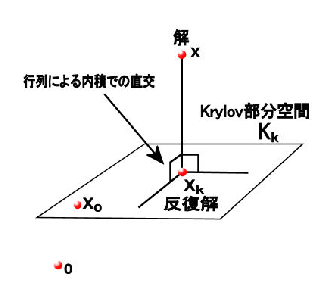
\includegraphics[width=6cm]{images/cg_projector.eps}
\caption{The iteration of conjugate gradient method(In Eucledian space)}
\end{center}
\end{figure}

Also, since the residual $\bi{r}_k$ at $k$ times iteration is $\bi{r}_k=\bi{A}(\bi{x}_k-\bi{x})$, the CG method can be said to find a solution as follows.

\begin{equation}
find \quad \bi{x}_k\in\bi{x}_0+{\cal K}_k 
\qquad 
so\;that
\qquad \qquad 
\bi{r}_k\quad\bot\quad{\cal K}_k
\end{equation}


This means that the solution  is looked for in the ${\cal K}_k+\bi{x}_0$ so that the residual $\bi{r}_k$ is orthogonal to the subspace ${\cal K}_k$.

The CG method has a deep relationship with the Lanczos method, which is a method of creating an orthonormal basis of Krylov subspace.



\section{Basic procedure}


\subsection{Increment of the solution}

Suppose that the increment of the solution from the $k$ iterative solution $\bi{x}_{k}$ to the $k+1$ iterative solution $\bi{x}_{k+1}$ is written using the coefficient $\alpha_k$ and the vector $\bi{p}_k$ as
%
\begin{equation}
\bi{x}_{k+1}-\bi{x}_{k}=\alpha_{k}\bi{p}_{k}.
\end{equation}
%
Since $\bi{p}$ determines the direction of solution increment, it is called \emph{search direction vector}.



Updating the solution to the $k+2$ iterative solution $\bi{x}_{k+2}$ The vector $\bi{p}_{k+1}$ is determined as follows using the residual $\bi{r}_{k+1}$ of the solution $\bi{x}_{k+1}$, the coefficient $\beta_k$, and the update vector $\bi{p}_k$ of the previous solution as follows


\begin{equation}
\bi{p}_{k+1}=\bi{r}_{k+1}+\beta_k\bi{p}_k
\end{equation}


Below, we explain how to determine the coefficients $\beta$ and $\alpha$.



\subsection{Determination of coefficient $\beta$}


From the previous discussion, in the CG method, the difference between the exact solution $\bi{x}$ and the iterative solution $\bi{x}_{k+1}$ was orthogonal in the $\bi{A}$ norm to the Krylov subspace ${\cal K}_{k+1}$. In other words,

\begin{equation}
\bi{x}_{k+1}-\bi{x}\quad\bot_{\bi{A}}\quad{\cal K}_{k+1}
\end{equation}


Therefore, since the difference $\bi{x}_{k+1}-\bi{x}$ from the exact solution lies in the orthogonal space in the Krylov subspace ${\cal K}_{k+1}$ and $\bi{A}$ norm, update the solution update vector $\bi{p}_{k+1}$ to the next iterative solution $\bi{x}_{k+2}$ from the orthogonal space with $\bi{A}$ norm to this ${\cal K}_{k+1}$ $\bi{x}_{k+2}$ should be closer to the exact solution.

As shown later, the previous search direction vector $\bi{p}_k$ of $\bi{p}_{k+1}$ is in the subspace ${\cal K}_{k+1}$ trying to make it orthogonal. In other words,

\begin{equation}
\bi{p}_k\in{\cal K}_{k+1}
\end{equation}


Therefore, in order for the search direction vector $\bi{p}_{k+1}$ to be orthogonal to ${\cal K}_{k+1}$ with the $\bi{A}$ norm, it is necessary to orthogonalize to the minimum $\bi{p}_k$ with $\bi{A}$ norm. In other words,

\begin {screen}
\begin{equation}
(\bi{p}_{k+1},\bi{p}_k)_{\bi{A}}=(\bi{p}_{k+1},\bi{A}\bi{p}_k)=0
\end{equation}
\end {screen}

As shown later, the search direction chosen as above is orthogonal not only to $\bi{p}_{k}$ but also to the ${\cal K}_{k+1}$ space by the $\bi{A}$ norm.

An expression that defines a search direction vector from the above residual and the previous search direction vector,


\begin{equation}
\bi{p}_{k+1}=\bi{r}_{k+1}+\beta_k\bi{p}_k
\end{equation}


, It means that a new search direction vector $\bi{p}_{k+1}$ can be obtained by projecting the residual difference $\bi{r}_{k+1}$ to the orthogonal space with the Krylov subspace ${\cal K}_{k+1}$ and $\bi{A}$ norm.

From this equation, we can determine $\beta$.

Substituting this expression into the expression $(\bi{p}_{k+1},\bi{A}\bi{p}_k)=0$ where the two search directions are orthogonal, the parameter $\beta$ becomes as follows. ~

\begin{equation}
\beta=-\frac{(\bi{r}_{k+1},\bi{A}\bi{p}_k)}{(\bi{p}_k,\bi{A}\bi{p}_k)}
\end{equation}



Furthermore, using the relational expression $(\bi{r}_i,\bi{r}_j)=0 \quad (\quad i\ne j\quad)$ of orthogonality of residuals to be described later,

\begin{equation}
(\bi{r}_{k+1},\bi{A}\bi{p}_k)=\left(\bi{r}_{k+1},-\frac{1}{\alpha_k}(\bi{r}_{k+1}-\bi{r}_k)\right)=-\frac{1}{\alpha_k}(\bi{r}_{k+1},\bi{r}_{k+1})
\end{equation}

\begin{equation}
(\bi{p}_k,\bi{A}\bi{p}_k)=\left(\bi{r}_k+\beta_{k-1}\bi{p}_{k-1},\bi{A}\bi{p}_k\right)=\left(\bi{r}_k,\bi{A}\bi{p}_k\right)=\left(\bi{r}_k,-\frac{1}{\alpha_k}(\bi{r}_{k+1}-\bi{r}_k)\right)=\frac{1}{\alpha_k}(\bi{r}_k,\bi{r}_k)
\end{equation}

As a result, the coefficient $\beta_k$ can be further expressed as follows.


\begin{equation}
\beta_k=-\frac{(\bi{r}_{k+1},\bi{A}\bi{p}_k)}{(\bi{p}_k,\bi{A}\bi{p}_k)}=-\frac{-\frac{1}{\alpha_k}(\bi{r}_{k+1},\bi{r}_{k+1})}{\frac{1}{\alpha_k}(\bi{r}_k,\bi{r}_k)}=\frac{(\bi{r}_{k+1},\bi{r}_{k+1})}{(\bi{r}_k,\bi{r}_k)}~
\end{equation}





\subsection{Determination of the coefficient $\alpha$}


The factor $\alpha$ is determined to minimize the potential $\phi_{k+1}$ in the next step.
The potential $\phi_{k+1}$ in the next step is

\begin{eqnarray}
\phi_{k+1} &=& \frac{1}{2}(\bi{x}_{k+1},\bi{A}\bi{x}_{k+1})-(\bi{x}_{k+1},\bi{f})\\
&=& \frac{1}{2}\left((\bi{x}_k+\alpha\bi{p}_k),\bi{A}(\bi{x}_k+\alpha\bi{p}_k)\right)-\left((\bi{x}_k+\alpha\bi{p}_k),\bi{f}\right)\\
&=& \left\{\frac{1}{2}(\bi{x}_k,\bi{A}\bi{x}_k)-(\bi{x}_k,\bi{f})\right\} + \alpha\left\{\frac{1}{2}(\bi{p}_k,\bi{A}\bi{x}_k)+\frac{1}{2}(\bi{x}_k,\bi{A}\bi{p}_k)-(\bi{p}_k,\bi{f})\right\}\\
&& + \alpha^2\left\{\frac{1}{2}(\bi{p}_k,\bi{A}\bi{p}_k)\right\}\\
&=& \phi_k+\alpha\left(\bi{p}_k,\frac{\bi{A}+\bi{A}^T}{2}\bi{x}_k-\bi{f}\right)+\alpha^2\left\{\frac{1}{2}(\bi{p}_k,\bi{A}\bi{p}_k)\right\}
\end{eqnarray}


Since the matrix $\bi{A}$ was symmetric, it is $\frac{\bi{A}+\bi{A}^T}{2}=\bi{A}$. Accordingly

\begin{eqnarray}
\phi_{k+1} = \phi_k+\alpha(\bi{p}_k,\bi{r}_k)+\alpha^2\left\{\frac{1}{2}(\bi{p}_k,\bi{A}\bi{p}_k)\right\}
\end{eqnarray}


When the potential $\phi_{k+1}$ takes the minimum value, the potential $\phi_{k+1}$ takes an extreme value

\begin{eqnarray}
\frac{\partial\phi_{k+1}}{\partial\alpha}=0
\end{eqnarray}


Therefore, when calculating this

\begin{eqnarray}
(\bi{p}_k,\bi{r}_k)=\alpha(\bi{p}_k,\bi{A}\bi{p}_k)
\end{eqnarray}


Therefore, the coefficient $\alpha$ becomes as follows.

\begin{eqnarray}
\alpha=\frac{(\bi{p}_k,\bi{r}_k)}{(\bi{p}_k,\bi{A}\bi{p}_k)}
\end{eqnarray}


Furthermore, using the relational expression $(\bi{r}_i,\bi{r}_j)=0 \quad (\quad  i\ne j\quad)$ of orthogonality of residuals to be described later,

\begin{eqnarray}
(\bi{p}_k,\bi{r}_k)=(\bi{r}_k-\beta_{k-1}\bi{p}_{k-1},\bi{r}_k)=(\bi{r}_k,\bi{r}_k)
\end{eqnarray}


As a result, the coefficient $\alpha_k$ can be further expressed as follows.

\begin{equation}
\alpha_k=\frac{(\bi{p}_k,\bi{r}_k)}{(\bi{p}_k,\bi{A}\bi{p}_k)}=\frac{(\bi{r}_k,\bi{r}_k)}{(\bi{p}_k,\bi{A}\bi{p}_k)}
\end{equation}



Using these, the algorithm of the CG method is as follows


\subsection{Algorithm (CG method)}

\begin{enumerate}
\item Compute $\bi{r}_0=\bi{b}-\bi{A}\bi{x}_0$, $\bi{p}_0=\bi{r}_0$
\item For $k=0,1,\ldots,m$, Do:
\begin{enumerate}
\item $\alpha_k=\frac{(\bi{r}_k,\bi{r}_k)}{(\bi{p}_k,\bi{A}\bi{p}_k)}$
\item $\bi{x}_{k+1}=\bi{x}_k+\alpha_k\bi{p}_k$
\item $\bi{r}_{k+1}=\bi{r}_k-\alpha_k\bi{A}\bi{p}_k$
\item $\beta_k=\frac{(\bi{r}_{k+1},\bi{r}_{k+1})}{(\bi{r}_k,\bi{r}_k)}$
\item $\bi{p}_{k+1}=\bi{r}_{k+1}+\beta_k\bi{p}_k$
\end{enumerate}
\item End Do
\end{enumerate}


% \ subsection {sample program}
% Discretization of the problem uses the finite element method.
% | ~ DOWNLOAD | [[CG.zip> http://ums.futene.net/wiki/SOL/CG.zip]] |

% OS: Windows XP, Windows 2000
% Development environment: VC ++ 2005
% Language: C ++


% \ subsubsection {Display convergence result}


% If you run the program, you should see a file called conv_history.dat in the folder where you started the program. This is a file that records the state of convergence and you can see it as a graph by typing the following command with gnuplot.

% set style data line
% set logscale y
% plot 'conv_history.dat'

% The following graph should be displayed.

% file: conv_history.png

% This convergence graph is detailed in [[Convergence of CG Method]].



\section{Krylov subspace and CG method}




\subsection{Proof: the CG method is a Krylov subspace method}

The CG method is a type of Krylov subspace method.
%
The Krylov subspace method is a method for finding an approximate solution that is closest to the solution in the Krylov subspace \eqref{eqn:krylov}.
%
Here we prove that the CG method is a Krylov subspace method.



We define subspaces $\bar{\cal K}_k,\tilde{\cal K}_k$ as:
%
\begin{eqnarray}
\bar{\cal K}_k &=&span\{\bi{p}_0,\bi{p}_1,\bi{p}_2,\cdots,\bi{p}_{k-1}\}\\
\tilde{\cal K}_k&=&span\{\bi{r}_0,\bi{r}_1,\bi{r}_2,\cdots,\bi{r}_{k-1}\}
\end{eqnarray}

We first prove these subspace are identical to the Krylov subspace \eqref{eqn:krylov} using the mathematical induction method.

\begin {itemize}
\item \textbf{$k=1$} \\
It is obvious from $\bi{r}_0=\bi{p}_0$.

\item \textbf{$k>1$} \\
Assume that it holds at $k$. In this case, it is checked whether or not it holds for k + 1. \\
$\bi{p}_k=\alpha(\bi{r}_k+\beta\bi{p}_{k-1})$, $\bi{p}_k\in\bar{\cal K}_{k+1}$, $\bi{r}_k\in\tilde{\cal K}_{k+1}$. \\
Also from the induction hypothesis $\bi{p}_{k-1}\in\bar{\cal K}_k=\tilde{\cal K}_k$ $\bar{\cal K}_{k+1}=\tilde{\cal K}_{k+1}$ holds. \\
$\bi{r}_k=\bi{r}_{k-1}+\alpha\bi{A}\bi{p}_{k-1}$, $\bi{r}_k\in\tilde{\cal K}_{k+1}$.
According to the induction hypothesis, since $\bi{r}_{k-1}\in\tilde{\cal K}_k={\cal K}_k$, $\bi{p}_{k-1}\in{\cal K}_k$, $\bi{A}\bi{p}_{k-1}\in{\cal K}{k+1}$, $\tilde{\cal K}_{k+1}={\cal K}_{k+1}$ is established \\
From the above we can say $\bar{\cal K}_{k+1}=\tilde{\cal K}_{k+1}={\cal K}_{k+1}$. \\
It can be seen that k + 1 also holds when assuming that the proposition is established in k.
\end{itemize}

From the above, the proposition was proved by mathematical induction.




By the way, given the solution $\bi{x}_k$ at the k-th iteration,
%
\begin{equation}
\bi{x}_k-\bi{x}_0=\sum_{i=0}^{k-1}\Delta\bi{x}_i=\sum_{i=0}^{k-1}\alpha_i\bi{p}_i.
\end{equation}
%
Because it is
%
\begin{equation}
\bi{x}_k-\bi{x}_0\in\bi{\cal K}_{k+1}=span\{\bi{r}_0,\bi{A}\bi{r}_0,\bi{A}^2\bi{r}_0,\cdots,\bi{A}^k\bi{r}_0\}
\end{equation}
%
Therefore, it can be seen that the CG method is a Krylov subspace method that searches for solutions in Krylov subspace. 





\subsection{Proof: orthogonality of the search direction vectors and residual vectors}

search direction vectors are $\bi{A}$-orthogonal and search direction vectors and residual are vector orthogonal


%
Prove using mathematical induction

\begin{itemize}

\item When $k=1$ \\
\begin{eqnarray}
(\bi{r}_1,\bi{p}_0)
&=&  (\bi{r}_0-\alpha\bi{A}\bi{p}_0,\bi{p}_0) = (\bi{r}_0,\bi{p}_0)-\frac{(\bi{r}_0,\bi{p}_0)}{(\bi{p}_0,\bi{A}\bi{p}_0)}(\bi{A}\bi{p}_0,\bi{p}_0)  =  0 \\
(\bi{A}\bi{p}_1,\bi{p}_0)
&=& (\bi{A}(\bi{r}_1-\beta\bi{p}_0),\bi{p}_0) = (\bi{A}\bi{r}_1,\bi{p}_0)-\frac{(\bi{r}_1,\bi{A}\bi{p}_0)}{(\bi{p}_0,\bi{A}\bi{p}_0)}(\bi{A}\bi{p}_0,\bi{p}_0) \\
&=& (\bi{r}_1,\bi{A}^T\bi{p}_0)-(\bi{r}_1,\bi{A}\bi{p}_0)=0
\end{eqnarray}\\
Here we used the condition $\bi{A}^T=\bi{A}$ that $\bi{A}$ is symmetric
\ item When $k>1$ \\
Assuming that it holds for $0\le{i}<{j}\le{k}$, in order to investigate whether $0\le{i}<{j}\le{k+1}$ also holds here, you can investigate whether it is true in $j=k+1$. In this case, considering the two cases of $i=k$ and $i\le{k}$ separately
\begin {itemize}
\item When $i=k$ \ \
\begin{eqnarray}
(\bi{r}_{k+1},\bi{p}_i)
&=&  (\bi{r}_{k+1},\bi{p}_k)  =  (\bi{r}_k-\alpha\bi{A}\bi{p}_k,\bi{p}_k) \\
&=& (\bi{r}_k,\bi{p}_k)-\frac{(\bi{r}_k,\bi{p}_k)}{(\bi{p}_k,\bi{A}\bi{p}_k)}(\bi{A}\bi{p}_k,\bi{p}_k)=0\\
(\bi{A}\bi{p}_{k+1},\bi{p}_i)
&=& (\bi{A}\bi{p}_{k+1},\bi{p}_k) = (\bi{A}(\bi{r}_{k+1}-\beta\bi{p}_k),\bi{p}_k) \\
&=& (\bi{A}\bi{r}_{k+1},\bi{p}_k)-\frac{(\bi{r}_{k+1},\bi{A}\bi{p}_k)}{(\bi{p}_k,\bi{A}\bi{p}_k)}(\bi{A}\bi{p}_k,\bi{p}_k) \\
&=& (\bi{r}_{k+1},\bi{A}^T\bi{p}_k)-(\bi{r}_{k+1},\bi{A}\bi{p}_k)=0
\end{eqnarray}

\item When $i<k$ \ \
\begin{eqnarray}
(\bi{r}_{k+1},\bi{p}_i)
&=&  (\bi{r}_k-\alpha\bi{A}\bi{p}_k,\bi{p}_i)\\
&=& (\bi{r}_k,\bi{p}_i)-\frac{(\bi{r}_k,\bi{p}_k)}{(\bi{p}_k,\bi{A}\bi{p}_k)}(\bi{A}\bi{p}_k,\bi{p}_i)=0\\
(\bi{A}\bi{p}_{k+1},\bi{p}_i)
&=&  (\bi{p}_{k+1},\bi{A}\bi{p}_i)  =  (\bi{r}_{k+1}-\beta\bi{p}_k,\bi{A}\bi{p}_i)  \\
&=&  (\bi{r}_{k+1},\bi{A}\bi{p}_i)-\beta(\bi{p}_k,\bi{A}\bi{p}_i)\\
&=&   \frac{1}{\alpha}(\bi{r}_{k+1},\bi{r}_i-\bi{r}_{i+1})-\beta(\bi{p}_k,\bi{A}\bi{p}_i)\\
&=&  \frac{1}{\alpha}\left(\bi{r}_{k+1},(\bi{p}_i+\beta\bi{p}_{i-1})-(\bi{p}_{i+1}+\beta\bi{p}_i)\right)-\beta(\bi{p}_k,\bi{A}\bi{p}_i)=0
\end{eqnarray}
\end {itemize}

\item So we can see that it also holds for $0\le{i}<{j}\le{k+1}$ since it is true even when $j=k+1$
\end {itemize}

The proposition is proved by using the mathematical induction method from the above



\subsection{Proof: all the residual vectors are orthogonal}


Prove by mathematical induction
\begin {itemize}
\item When $k=1$ \\
\begin{equation}
(\bi{r}_0,\bi{r}_1)=(\bi{p}_0,\bi{r}_1)=0
\end{equation}
\item When $k>1$ \ \
Assuming that it holds for $0\le{i}<{j}\le{k}$, in order to investigate whether $0\le{i}<{j}\le{k+1}$ also holds here, you can check whether it is true in $j=k+1$. \\
\begin{eqnarray}
(\bi{r}_i,\bi{r}_{k+1})
&=&  (\bi{r}_i,\bi{r}_k-\alpha\bi{A}\bi{p}_k)  =  (\bi{r}_i,\bi{r}_k)-\alpha(\bi{A}\bi{p}_k,\bi{r}_i)\\
&=&  (\bi{r}_i,\bi{r}_k)-\alpha(\bi{A}\bi{p}_k,\bi{p}_i+\beta\bi{p}_{i-1})  =  0
\end{eqnarray}\\
Therefore, it can be seen that $0\le{i}<{j}\le{k+1}$ also holds since it holds even in $j=k+1$
\end {itemize}

The proposition is proved by using the mathematical induction method from the above


\subsection{CG method converge in finite iterations (only theoretically!)}

We shows that the CG method always converges with iteration of n solution from the condition that the residual $r$ is orthogonal.

Here, it is found that the column $\bi{r}_i$ of the residual vector is a linear independent vector orthogonal to each other. Since the maximum value of the number of linearly independent vectors is the number of dimensions $n$ of the vector, it can be seen that the number of columns of the residual vector does not become larger than the dimension number $n$ of the vector.
%
\begin{screen}
\textbf{CG method always converges with the number of iterations of vector dimension $n$ or less}
\end{screen}

However, this is only in theory where there is no error in the floating point number computation.
%
The CG method is strongly influenced by the rounding error, so on the calculator the CG method never converges per n iterations. 
%
Using the Chebyshev inequality, more accurate convergence conditions can be obtained.


\if0
\section{CG method in complex matrix}

If the coefficients are complex numbers, the coefficient matrix $A$ is not a symmetric matrix but must be Hermetian Matrix. That is


\begin{equation}
A^*=A
\end{equation}



In this case, the inner product $(p,Ap)$ is a real number.
Also, all eigenvalues ​​are real numbers.

If the coefficient matrix is ​​not a Hermitian matrix but a symmetric matrix, it can be solved using the Conjugate Orgonal Conjugate Gradient Method (COCG) method.

If not, use the CGNR method (Conjugate Non-Linear Method), etc.


% \ subsection {CGNR method}


% / / In the CGNR method, solve the equation multiplied by & mimetex (\ b {A} ^ \ section {); from the left to the equation to be solved as follows: / mimetex (\ b {A} ^ \ {{ b {A} \ b {x} = \ b {A} ^ \ section {\ b {b});}


% // coefficient matrix & mimetex (A); is a Hermitian matrix like & mimetex (A ^ \ section {A);,}

% // It can adapt and solve the CG method.
% // However, the CGNR method is inefficient compared to the original CG method.
% // Because the product of Hermitian matrix and vector is necessary compared with CG method.
% // The condition number of the coefficient matrix (Condition Number) is squared
% // That is, if the condition number of $\bi{A}$ is $\kappa$,

The condition number of% // & mimetex (A ^ \ section {A); is & mimetex (\ kappa ^ 2);

% // It will become bigger.

% / / \ section {Relationship between Lancoz method and CG method}


% // \ section {CG method and steepest descent method}
\fi




\if0
\section{What I referred to}

\ cite {hestenes-methods}, \ cite {wiki_conj_grad}, \ cite {hp_tuchiya_cg_steep}, \ cite {hppdf_shewchek_cg}

\ bibliographystyle {tipsj}
\ bibliography {../../ main}
\fi


\end{document}
